\documentclass[a4paper,12pt]{article}
\usepackage[utf8]{inputenc}
\usepackage[T1]{fontenc}
\usepackage[margin=1in]{geometry}
\usepackage{amsmath, amssymb, mathtools}
\usepackage{tcolorbox}
\usepackage{enumitem}
\usepackage{fancyhdr}
\usepackage{titlesec}
\usepackage{tikz}
\usepackage{pgfplots}
\usepackage{hyperref}
\usepackage{longtable}
\usepackage{array}

\pgfplotsset{compat=1.18}

% Header and Footer
\pagestyle{fancy}
\fancyhf{}
\fancyhead[L]{Mathematics-I (DI01000021)}
\fancyhead[R]{Winter 2024 Solution}
\fancyfoot[C]{\thepage}

% Title Formatting
\titleformat{\section}{\large\bfseries}{\thesection}{1em}{}
\titleformat{\subsection}{\bfseries}{\thesubsection}{1em}{}

% Custom Environments
\newtcolorbox{solutionbox}{
    colback=gray!5,
    colframe=gray!40,
    boxrule=0.5pt,
    arc=2pt,
    left=5pt, right=5pt, top=5pt, bottom=5pt
}

\begin{document}

\begin{center}
    {\Large\textbf{Mathematics-I (DI01000021) - Winter 2024 Solution}}\\[0.5cm]
    \textit{Date: 2025-01-02}
\end{center}

\section*{Q.1 [14 marks]}
\textbf{Fill in the blanks/MCQs using appropriate choice from the given options.}

\subsection*{Q1.1 [1 mark]}
$\begin{vmatrix} 5 & 1 \\ 2 & 3 \end{vmatrix} = $ \underline{\hspace{2cm}}

\textbf{Answer}: b. 13

\begin{solutionbox}
\textbf{Solution}:\\
For 2×2 determinant $\begin{vmatrix} a & b \\ c & d \end{vmatrix} = ad - bc$\\
$\begin{vmatrix} 5 & 1 \\ 2 & 3 \end{vmatrix} = (5 \times 3) - (1 \times 2) = 15 - 2 = 13$
\end{solutionbox}

\subsection*{Q1.2 [1 mark]}
If $\begin{vmatrix} x & 1 \\ 2 & 1 \end{vmatrix} = 0$ then $x = $ \underline{\hspace{2cm}}

\textbf{Answer}: b. 2

\begin{solutionbox}
\textbf{Solution}:\\
$\begin{vmatrix} x & 1 \\ 2 & 1 \end{vmatrix} = x \times 1 - 1 \times 2 = x - 2 = 0$\\
Therefore, $x = 2$
\end{solutionbox}

\subsection*{Q1.3 [1 mark]}
If $f(x) = x^2$ then $f(-1) = $ \underline{\hspace{2cm}}

\textbf{Answer}: a. 1

\begin{solutionbox}
\textbf{Solution}:\\
$f(x) = x^2$\\
$f(-1) = (-1)^2 = 1$
\end{solutionbox}

\subsection*{Q1.4 [1 mark]}
$\log_{10} 1 = $ \underline{\hspace{2cm}}

\textbf{Answer}: b. 0

\begin{solutionbox}
\textbf{Solution}:\\
By logarithm property: $\log_a 1 = 0$ for any base $a > 0$\\
Therefore, $\log_{10} 1 = 0$
\end{solutionbox}

\subsection*{Q1.5 [1 mark]}
$\sin \frac{\pi}{2} + \cos \frac{\pi}{2} = $ \underline{\hspace{2cm}}

\textbf{Answer}: c. 1

\begin{solutionbox}
\textbf{Solution}:\\
$\sin \frac{\pi}{2} = 1$ and $\cos \frac{\pi}{2} = 0$\\
Therefore, $\sin \frac{\pi}{2} + \cos \frac{\pi}{2} = 1 + 0 = 1$
\end{solutionbox}

\subsection*{Q1.6 [1 mark]}
$\tan^{-1}(1) = $ \underline{\hspace{2cm}}

\textbf{Answer}: a. $\frac{\pi}{4}$

\begin{solutionbox}
\textbf{Solution}:\\
$\tan \frac{\pi}{4} = 1$\\
Therefore, $\tan^{-1}(1) = \frac{\pi}{4}$
\end{solutionbox}

\subsection*{Q1.7 [1 mark]}
$\frac{2\pi}{3}$ radian = \underline{\hspace{2cm}} degree

\textbf{Answer}: d. 120

\begin{solutionbox}
\textbf{Solution}:\\
To convert radians to degrees: $\text{degrees} = \text{radians} \times \frac{180}{\pi}$\\
$\frac{2\pi}{3} \times \frac{180}{\pi} = \frac{2 \times 180}{3} = \frac{360}{3} = 120^\circ$
\end{solutionbox}

\subsection*{Q1.8 [1 mark]}
$\hat{i} \times \hat{j} = $ \underline{\hspace{2cm}}

\textbf{Answer}: c. $\hat{k}$

\begin{solutionbox}
\textbf{Solution}:\\
By right-hand rule for cross product:\\
$\hat{i} \times \hat{j} = \hat{k}$
\end{solutionbox}

\subsection*{Q1.9 [1 mark]}
$|\hat{i} + \hat{j} + \hat{k}| = $ \underline{\hspace{2cm}}

\textbf{Answer}: d. $\sqrt{3}$

\begin{solutionbox}
\textbf{Solution}:\\
$|\hat{i} + \hat{j} + \hat{k}| = \sqrt{1^2 + 1^2 + 1^2} = \sqrt{3}$
\end{solutionbox}

\subsection*{Q1.10 [1 mark]}
Slope of line $2x + y - 3 = 0$ is \underline{\hspace{2cm}}

\textbf{Answer}: a. -2

\begin{solutionbox}
\textbf{Solution}:\\
Convert to slope-intercept form: $y = -2x + 3$\\
Slope = coefficient of $x = -2$
\end{solutionbox}

\subsection*{Q1.11 [1 mark]}
Radius of circle $x^2 + y^2 = 81$ is \underline{\hspace{2cm}}

\textbf{Answer}: b. 9

\begin{solutionbox}
\textbf{Solution}:\\
Standard form: $x^2 + y^2 = r^2$\\
Here, $r^2 = 81$, so $r = 9$
\end{solutionbox}

\subsection*{Q1.12 [1 mark]}
$\lim_{n \to \infty} \frac{1}{n} = $ \underline{\hspace{2cm}}

\textbf{Answer}: c. 0

\begin{solutionbox}
\textbf{Solution}:\\
As $n$ approaches infinity, $\frac{1}{n}$ approaches 0
\end{solutionbox}

\subsection*{Q1.13 [1 mark]}
$\lim_{x \to 1} (x^2 + x + 1) = $ \underline{\hspace{2cm}}

\textbf{Answer}: a. 3

\begin{solutionbox}
\textbf{Solution}:\\
Direct substitution: $(1)^2 + (1) + 1 = 1 + 1 + 1 = 3$
\end{solutionbox}

\subsection*{Q1.14 [1 mark]}
$\lim_{\theta \to 0} \frac{\tan \theta}{\theta} = $ \underline{\hspace{2cm}}

\textbf{Answer}: b. 1

\begin{solutionbox}
\textbf{Solution}:\\
This is a standard limit: $\lim_{\theta \to 0} \frac{\tan \theta}{\theta} = 1$
\end{solutionbox}

\section*{Q.2 (A) [6 marks]}
\textbf{Attempt any two}

\subsection*{Q2.1 [3 marks]}
\textbf{Find the value of $\begin{vmatrix} 1 & 3 & 1 \\ 2 & -1 & 0 \\ 4 & -2 & 5 \end{vmatrix}$}

\begin{solutionbox}
\textbf{Solution}:\\
Using expansion along second row (has zero):\\
$= -2\begin{vmatrix} 3 & 1 \\ -2 & 5 \end{vmatrix} + (-1)\begin{vmatrix} 1 & 1 \\ 4 & 5 \end{vmatrix} + 0$\\
$= -2(15 + 2) - 1(5 - 4)$\\
$= -2(17) - 1(1)$\\
$= -34 - 1 = -35$

\begin{tabular}{|l|l|l|}
\hline
\textbf{Step} & \textbf{Calculation} & \textbf{Result} \\
\hline
Minor 1 & $(3 \times 5) - (1 \times -2)$ & 17 \\
\hline
Minor 2 & $(1 \times 5) - (1 \times 4)$ & 1 \\
\hline
Final & $-2(17) - 1(1)$ & -35 \\
\hline
\end{tabular}
\end{solutionbox}

\subsection*{Q2.2 [3 marks]}
\textbf{If $f(x) = x^3 + 5$ then find $f(0)$, $f(1)$ and $f(-1)$}

\begin{solutionbox}
\textbf{Solution}:\\
Given: $f(x) = x^3 + 5$\\
$f(0) = (0)^3 + 5 = 0 + 5 = 5$\\
$f(1) = (1)^3 + 5 = 1 + 5 = 6$\\
$f(-1) = (-1)^3 + 5 = -1 + 5 = 4$

\begin{tabular}{|l|l|l|}
\hline
\textbf{Input} & \textbf{Calculation} & \textbf{Output} \\
\hline
$f(0)$ & $0^3 + 5$ & 5 \\
\hline
$f(1)$ & $1^3 + 5$ & 6 \\
\hline
$f(-1)$ & $(-1)^3 + 5$ & 4 \\
\hline
\end{tabular}
\end{solutionbox}

\subsection*{Q2.3 [3 marks]}
\textbf{Prove that $\tan^{-1}\left(\frac{1}{2}\right) + \tan^{-1}\left(\frac{1}{3}\right) = \frac{\pi}{4}$}

\begin{solutionbox}
\textbf{Solution}:\\
Using formula: $\tan^{-1}a + \tan^{-1}b = \tan^{-1}\left(\frac{a+b}{1-ab}\right)$\\
Let $a = \frac{1}{2}$, $b = \frac{1}{3}$\\
$\tan^{-1}\left(\frac{1}{2}\right) + \tan^{-1}\left(\frac{1}{3}\right) = \tan^{-1}\left(\frac{\frac{1}{2} + \frac{1}{3}}{1 - \frac{1}{2} \times \frac{1}{3}}\right)$\\
$= \tan^{-1}\left(\frac{\frac{5}{6}}{1 - \frac{1}{6}}\right) = \tan^{-1}\left(\frac{\frac{5}{6}}{\frac{5}{6}}\right) = \tan^{-1}(1) = \frac{\pi}{4}$\\
Hence proved.
\end{solutionbox}

\section*{Q.2 (B) [8 marks]}
\textbf{Attempt any two}

\subsection*{Q2.1 [4 marks]}
\textbf{If $f(x) = \frac{x-1}{x+1}$ then prove that $f(x) \cdot f(-x) = 1$}

\begin{solutionbox}
\textbf{Solution}:\\
Given: $f(x) = \frac{x-1}{x+1}$\\
First find $f(-x)$:\\
$f(-x) = \frac{(-x)-1}{(-x)+1} = \frac{-x-1}{-x+1} = \frac{-(x+1)}{-(x-1)} = \frac{x+1}{x-1}$\\
Now calculate $f(x) \cdot f(-x)$:\\
$f(x) \cdot f(-x) = \frac{x-1}{x+1} \cdot \frac{x+1}{x-1} = \frac{(x-1)(x+1)}{(x+1)(x-1)} = 1$\\
Hence proved.
\end{solutionbox}

\subsection*{Q2.2 [4 marks]}
\textbf{If $\log\left(\frac{x+y}{2}\right) = \frac{1}{2}(\log x + \log y)$ then prove that $x = y$}

\begin{solutionbox}
\textbf{Solution}:\\
Given: $\log\left(\frac{x+y}{2}\right) = \frac{1}{2}(\log x + \log y)$\\
Using logarithm properties:\\
$\frac{1}{2}(\log x + \log y) = \frac{1}{2}\log(xy) = \log\sqrt{xy}$\\
So: $\log\left(\frac{x+y}{2}\right) = \log\sqrt{xy}$\\
Taking antilog: $\frac{x+y}{2} = \sqrt{xy}$\\
Squaring both sides: $\left(\frac{x+y}{2}\right)^2 = xy$\\
$\frac{(x+y)^2}{4} = xy$\\
$(x+y)^2 = 4xy$\\
$x^2 + 2xy + y^2 = 4xy$\\
$x^2 - 2xy + y^2 = 0$\\
$(x-y)^2 = 0$\\
Therefore, $x = y$. Hence proved.
\end{solutionbox}

\subsection*{Q2.3 [4 marks]}
\textbf{Solve $\log(x+3) + \log(x-3) = \log 27$}

\begin{solutionbox}
\textbf{Solution}:\\
Given: $\log(x+3) + \log(x-3) = \log 27$\\
Using logarithm property: $\log a + \log b = \log(ab)$\\
$\log[(x+3)(x-3)] = \log 27$\\
Taking antilog: $(x+3)(x-3) = 27$\\
$x^2 - 9 = 27$\\
$x^2 = 36$\\
$x = \pm 6$\\
\textbf{Check validity:}\\
- For $x = 6$: $x+3 = 9 > 0$ and $x-3 = 3 > 0$ \checkmark\\
- For $x = -6$: $x+3 = -3 < 0$ (invalid for logarithm)\\
Therefore, $x = 6$
\end{solutionbox}

\section*{Q.3 (A) [6 marks]}
\textbf{Attempt any two}

\subsection*{Q3.1 [3 marks]}
\textbf{Prove that $\frac{\sin\left(\frac{\pi}{2}+\theta\right)}{\cos(\pi-\theta)} + \frac{\tan(\pi-\theta)}{\cot\left(\frac{3\pi}{2}-\theta\right)} + \frac{\text{cosec}\left(\frac{\pi}{2}-\theta\right)}{\sec(\pi+\theta)} = -3$}

\begin{solutionbox}
\textbf{Solution}:\\
Using trigonometric identities:\\
$\sin\left(\frac{\pi}{2}+\theta\right) = \cos\theta$\\
$\cos(\pi-\theta) = -\cos\theta$\\
$\tan(\pi-\theta) = -\tan\theta$\\
$\cot\left(\frac{3\pi}{2}-\theta\right) = \tan\theta$\\
$\text{cosec}\left(\frac{\pi}{2}-\theta\right) = \sec\theta$\\
$\sec(\pi+\theta) = -\sec\theta$\\
Substituting:\\
$\frac{\cos\theta}{-\cos\theta} + \frac{-\tan\theta}{\tan\theta} + \frac{\sec\theta}{-\sec\theta}$\\
$= -1 + (-1) + (-1) = -3$\\
Hence proved.
\end{solutionbox}

\subsection*{Q3.2 [3 marks]}
\textbf{Prove that $\tan 55^\circ = \frac{\cos 10^\circ + \sin 10^\circ}{\cos 10^\circ - \sin 10^\circ}$}

\begin{solutionbox}
\textbf{Solution}:\\
We know that $\tan 55^\circ = \tan(45^\circ + 10^\circ)$\\
Using formula: $\tan(A + B) = \frac{\tan A + \tan B}{1 - \tan A \tan B}$\\
$\tan 55^\circ = \frac{\tan 45^\circ + \tan 10^\circ}{1 - \tan 45^\circ \tan 10^\circ} = \frac{1 + \tan 10^\circ}{1 - \tan 10^\circ}$\\
Now, $\tan 10^\circ = \frac{\sin 10^\circ}{\cos 10^\circ}$\\
$\tan 55^\circ = \frac{1 + \frac{\sin 10^\circ}{\cos 10^\circ}}{1 - \frac{\sin 10^\circ}{\cos 10^\circ}} = \frac{\cos 10^\circ + \sin 10^\circ}{\cos 10^\circ - \sin 10^\circ}$\\
Hence proved.
\end{solutionbox}

\subsection*{Q3.3 [3 marks]}
\textbf{If $\vec{a} = 2\hat{i} + 3\hat{j} + \hat{k}$, $\vec{b} = \hat{i} + \hat{j} + \hat{k}$ and $\vec{c} = 3\hat{i} + \hat{j} + \hat{k}$ then find $2\vec{a} + \vec{b} - \vec{c}$}

\begin{solutionbox}
\textbf{Solution}:\\
Given:\\
$\vec{a} = 2\hat{i} + 3\hat{j} + \hat{k}$\\
$\vec{b} = \hat{i} + \hat{j} + \hat{k}$\\
$\vec{c} = 3\hat{i} + \hat{j} + \hat{k}$\\
$2\vec{a} = 2(2\hat{i} + 3\hat{j} + \hat{k}) = 4\hat{i} + 6\hat{j} + 2\hat{k}$\\
$2\vec{a} + \vec{b} - \vec{c} = (4\hat{i} + 6\hat{j} + 2\hat{k}) + (\hat{i} + \hat{j} + \hat{k}) - (3\hat{i} + \hat{j} + \hat{k})$\\
$= (4 + 1 - 3)\hat{i} + (6 + 1 - 1)\hat{j} + (2 + 1 - 1)\hat{k}$\\
$= 2\hat{i} + 6\hat{j} + 2\hat{k}$
\end{solutionbox}

\section*{Q.3 (B) [8 marks]}
\textbf{Attempt any two}

\subsection*{Q3.1 [4 marks]}
\textbf{Prove that $\frac{\sin(x-y)}{\cos x \cos y} + \frac{\sin(y-z)}{\cos y \cos z} + \frac{\sin(z-x)}{\cos z \cos x} = 0$}

\begin{solutionbox}
\textbf{Solution}:\\
Using identity: $\sin(A-B) = \sin A \cos B - \cos A \sin B$\\
$\frac{\sin(x-y)}{\cos x \cos y} = \frac{\sin x \cos y - \cos x \sin y}{\cos x \cos y} = \tan x - \tan y$\\
Similarly:\\
$\frac{\sin(y-z)}{\cos y \cos z} = \tan y - \tan z$\\
$\frac{\sin(z-x)}{\cos z \cos x} = \tan z - \tan x$\\
Adding all three:\\
$(\tan x - \tan y) + (\tan y - \tan z) + (\tan z - \tan x) = 0$\\
Hence proved.
\end{solutionbox}

\subsection*{Q3.2 [4 marks]}
\textbf{Draw graph of $y = \cos x$ for $0 \leq x \leq \pi$}

\begin{solutionbox}
\textbf{Solution}:\\
\begin{center}
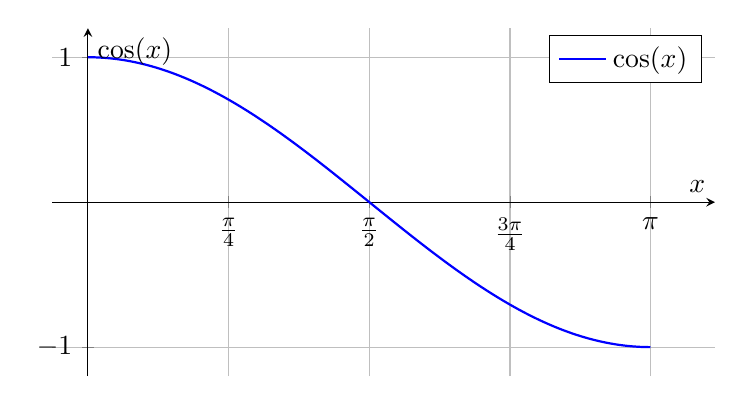
\begin{tikzpicture}
\begin{axis}[
    axis lines = center,
    xlabel = $x$,
    ylabel = {$\cos(x)$},
    ymin=-1.2, ymax=1.2,
    xmin=-0.2, xmax=3.5,
    xtick={0, 0.785, 1.57, 2.356, 3.14},
    xticklabels={0, $\frac{\pi}{4}$, $\frac{\pi}{2}$, $\frac{3\pi}{4}$, $\pi$},
    ytick={-1, 0, 1},
    grid=both,
    width=10cm, height=6cm
]
\addplot [
    domain=0:3.14, 
    samples=100, 
    color=blue,
    thick
]
{cos(deg(x))};
\addlegendentry{$\cos(x)$}
\end{axis}
\end{tikzpicture}
\end{center}

\textbf{Table of values:}
\begin{tabular}{|l|l|l|l|l|l|}
\hline
$x$ & 0 & $\pi/4$ & $\pi/2$ & $3\pi/4$ & $\pi$ \\
\hline
$y$ & 1 & $\sqrt{2}/2$ & 0 & $-\sqrt{2}/2$ & -1 \\
\hline
\end{tabular}
\end{solutionbox}

\subsection*{Q3.3 [4 marks]}
\textbf{Find equation of line passing through (1, 2) and (-3, 1)}

\begin{solutionbox}
\textbf{Solution}:\\
Given points: $(x_1, y_1) = (1, 2)$ and $(x_2, y_2) = (-3, 1)$\\
Slope: $m = \frac{y_2 - y_1}{x_2 - x_1} = \frac{1 - 2}{-3 - 1} = \frac{-1}{-4} = \frac{1}{4}$\\
Using point-slope form: $y - y_1 = m(x - x_1)$\\
$y - 2 = \frac{1}{4}(x - 1)$\\
$4(y - 2) = x - 1$\\
$4y - 8 = x - 1$\\
$x - 4y + 7 = 0$\\
\textbf{Equation:} $x - 4y + 7 = 0$
\end{solutionbox}

\section*{Q.4 (A) [6 marks]}
\textbf{Attempt any two}

\subsection*{Q4.1 [3 marks]}
\textbf{Find unit vector perpendicular to $\vec{a} = \hat{i} - 3\hat{j} + \hat{k}$ and $\vec{b} = 2\hat{i} + \hat{j} + 2\hat{k}$}

\begin{solutionbox}
\textbf{Solution}:\\
Cross product: $\vec{a} \times \vec{b} = \begin{vmatrix} \hat{i} & \hat{j} & \hat{k} \\ 1 & -3 & 1 \\ 2 & 1 & 2 \end{vmatrix}$\\
$= \hat{i}[(-3)(2) - (1)(1)] - \hat{j}[(1)(2) - (1)(2)] + \hat{k}[(1)(1) - (-3)(2)]$\\
$= \hat{i}(-6-1) - \hat{j}(2-2) + \hat{k}(1+6)$\\
$= -7\hat{i} + 0\hat{j} + 7\hat{k}$\\
Magnitude: $|\vec{a} \times \vec{b}| = \sqrt{(-7)^2 + 0^2 + 7^2} = \sqrt{49 + 49} = 7\sqrt{2}$\\
Unit vector: $\hat{n} = \frac{-7\hat{i} + 7\hat{k}}{7\sqrt{2}} = \frac{-\hat{i} + \hat{k}}{\sqrt{2}}$
\end{solutionbox}

\subsection*{Q4.2 [3 marks]}
\textbf{Forces (1, 2, 1) and (2, -1, 3) act on a particle and the particle moves from point (2, 3, 1) to (4, 6, 2). Find the work done.}

\begin{solutionbox}
\textbf{Solution}:\\
Resultant force: $\vec{F} = (1, 2, 1) + (2, -1, 3) = (3, 1, 4)$\\
Displacement: $\vec{s} = (4, 6, 2) - (2, 3, 1) = (2, 3, 1)$\\
Work done: $W = \vec{F} \cdot \vec{s} = (3)(2) + (1)(3) + (4)(1) = 6 + 3 + 4 = 13$ units
\end{solutionbox}

\subsection*{Q4.3 [3 marks]}
\textbf{Show that lines $2x - 3y + 5 = 0$ and $8x - 12y - 3 = 0$ are parallel lines.}

\begin{solutionbox}
\textbf{Solution}:\\
For line $2x - 3y + 5 = 0$: slope $m_1 = \frac{2}{3}$\\
For line $8x - 12y - 3 = 0$: slope $m_2 = \frac{8}{12} = \frac{2}{3}$\\
Since $m_1 = m_2 = \frac{2}{3}$, the lines are parallel.

\begin{tabular}{|l|l|l|}
\hline
\textbf{Line} & \textbf{Standard Form} & \textbf{Slope} \\
\hline
Line 1 & $2x - 3y + 5 = 0$ & $\frac{2}{3}$ \\
\hline
Line 2 & $8x - 12y - 3 = 0$ & $\frac{2}{3}$ \\
\hline
\end{tabular}
\end{solutionbox}

\section*{Q.4 (B) [8 marks]}
\textbf{Attempt any two}

\subsection*{Q4.1 [4 marks]}
\textbf{Show that angle between $\vec{a} = \hat{i} + \hat{j} - \hat{k}$ and $\vec{b} = 2\hat{i} - 2\hat{j} + \hat{k}$ is $\sin^{-1}\left(\frac{\sqrt{26}}{27}\right)$}

\begin{solutionbox}
\textbf{Solution}:\\
$\vec{a} \cdot \vec{b} = (1)(2) + (1)(-2) + (-1)(1) = 2 - 2 - 1 = -1$\\
$|\vec{a}| = \sqrt{1^2 + 1^2 + (-1)^2} = \sqrt{3}$\\
$|\vec{b}| = \sqrt{2^2 + (-2)^2 + 1^2} = \sqrt{9} = 3$\\
$\cos\theta = \frac{\vec{a} \cdot \vec{b}}{|\vec{a}||\vec{b}|} = \frac{-1}{\sqrt{3} \times 3} = \frac{-1}{3\sqrt{3}}$\\
$\sin^2\theta = 1 - \cos^2\theta = 1 - \frac{1}{27} = \frac{26}{27}$\\
Therefore, $\sin\theta = \frac{\sqrt{26}}{3\sqrt{3}} = \frac{\sqrt{26}}{\sqrt{27}}$\\
Hence, $\theta = \sin^{-1}\left(\frac{\sqrt{26}}{\sqrt{27}}\right)$
\end{solutionbox}

\subsection*{Q4.2 [4 marks]}
\textbf{If $\vec{a} = (1, 1, 1)$, $\vec{b} = (2, 0, 1)$ and $\vec{c} = (-2, 1, 0)$ then find $\vec{a} \cdot (\vec{b} \times \vec{c})$}

\begin{solutionbox}
\textbf{Solution}:\\
First find $\vec{b} \times \vec{c}$:\\
$\vec{b} \times \vec{c} = \begin{vmatrix} \hat{i} & \hat{j} & \hat{k} \\ 2 & 0 & 1 \\ -2 & 1 & 0 \end{vmatrix}$\\
$= \hat{i}(0 \times 0 - 1 \times 1) - \hat{j}(2 \times 0 - 1 \times (-2)) + \hat{k}(2 \times 1 - 0 \times (-2))$\\
$= \hat{i}(-1) - \hat{j}(2) + \hat{k}(2)$\\
$= -\hat{i} - 2\hat{j} + 2\hat{k}$\\
Now find $\vec{a} \cdot (\vec{b} \times \vec{c})$:\\
$\vec{a} \cdot (\vec{b} \times \vec{c}) = (1, 1, 1) \cdot (-1, -2, 2)$\\
$= (1)(-1) + (1)(-2) + (1)(2) = -1 - 2 + 2 = -1$
\end{solutionbox}

\subsection*{Q4.3 [4 marks]}
\textbf{Evaluate $\lim_{\theta \to 0} \frac{\sin 4\theta}{\theta}$}

\begin{solutionbox}
\textbf{Solution}:\\
$\lim_{\theta \to 0} \frac{\sin 4\theta}{\theta} = \lim_{\theta \to 0} \frac{\sin 4\theta}{4\theta} \times 4$\\
Using standard limit $\lim_{x \to 0} \frac{\sin x}{x} = 1$:\\
Let $u = 4\theta$, then as $\theta \to 0$, $u \to 0$\\
$\lim_{\theta \to 0} \frac{\sin 4\theta}{4\theta} = \lim_{u \to 0} \frac{\sin u}{u} = 1$\\
Therefore, $\lim_{\theta \to 0} \frac{\sin 4\theta}{\theta} = 4 \times 1 = 4$
\end{solutionbox}

\section*{Q.5 (A) [6 marks]}
\textbf{Attempt any two}

\subsection*{Q5.1 [3 marks]}
\textbf{Evaluate $\lim_{x \to 9} \frac{x^2 - 81}{x - 9}$}

\begin{solutionbox}
\textbf{Solution}:\\
Direct substitution gives $\frac{0}{0}$ form.\\
Factor the numerator: $x^2 - 81 = (x-9)(x+9)$\\
$\lim_{x \to 9} \frac{x^2 - 81}{x - 9} = \lim_{x \to 9} \frac{(x-9)(x+9)}{x-9}$\\
$= \lim_{x \to 9} (x+9) = 9 + 9 = 18$
\end{solutionbox}

\subsection*{Q5.2 [3 marks]}
\textbf{Evaluate $\lim_{x \to \infty} \left(1 + \frac{3}{x}\right)^{2x}$}

\begin{solutionbox}
\textbf{Solution}:\\
Let $y = \left(1 + \frac{3}{x}\right)^{2x}$\\
Taking natural logarithm:\\
$\ln y = 2x \ln\left(1 + \frac{3}{x}\right)$\\
As $x \to \infty$, $\frac{3}{x} \to 0$\\
Using $\ln(1+u) \approx u$ for small $u$:\\
$\ln y = 2x \times \frac{3}{x} = 6$\\
Therefore, $y = e^6$
\end{solutionbox}

\subsection*{Q5.3 [3 marks]}
\textbf{Evaluate $\lim_{x \to 1} \frac{x - 1}{x^2 + x - 2}$}

\begin{solutionbox}
\textbf{Solution}:\\
Factor the denominator: $x^2 + x - 2 = (x+2)(x-1)$\\
$\lim_{x \to 1} \frac{x - 1}{x^2 + x - 2} = \lim_{x \to 1} \frac{x-1}{(x+2)(x-1)}$\\
$= \lim_{x \to 1} \frac{1}{x+2} = \frac{1}{1+2} = \frac{1}{3}$
\end{solutionbox}

\section*{Q.5 (B) [8 marks]}
\textbf{Attempt any two}

\subsection*{Q5.1 [4 marks]}
\textbf{Find the equation of line passing through the point (2, -3) and having slope 4.}

\begin{solutionbox}
\textbf{Solution}:\\
Using point-slope form: $y - y_1 = m(x - x_1)$\\
Given: $(x_1, y_1) = (2, -3)$ and slope $m = 4$\\
$y - (-3) = 4(x - 2)$\\
$y + 3 = 4x - 8$\\
$y = 4x - 11$\\
\textbf{Equation:} $y = 4x - 11$ or $4x - y - 11 = 0$
\end{solutionbox}

\subsection*{Q5.2 [4 marks]}
\textbf{For what value of m, lines $7x + y - 1 = 0$ and $3x - my + 2 = 0$ are perpendicular to each other.}

\begin{solutionbox}
\textbf{Solution}:\\
For perpendicular lines, product of slopes = -1\\
For line $7x + y - 1 = 0$: slope $m_1 = -7$\\
For line $3x - my + 2 = 0$: slope $m_2 = \frac{3}{m}$\\
Condition: $m_1 \times m_2 = -1$\\
$(-7) \times \frac{3}{m} = -1$\\
$\frac{-21}{m} = -1$\\
$21 = m$\\
Therefore, $m = 21$
\end{solutionbox}

\subsection*{Q5.3 [4 marks]}
\textbf{Find the centre and radius of the circle $4x^2 + 4y^2 + 8x - 12y - 3 = 0$}

\begin{solutionbox}
\textbf{Solution}:\\
First, divide by 4 to get standard form:\\
$x^2 + y^2 + 2x - 3y - \frac{3}{4} = 0$\\
Complete the square for x and y terms:\\
$x^2 + 2x = (x+1)^2 - 1$\\
$y^2 - 3y = \left(y - \frac{3}{2}\right)^2 - \frac{9}{4}$\\
Substituting:\\
$(x+1)^2 - 1 + \left(y - \frac{3}{2}\right)^2 - \frac{9}{4} - \frac{3}{4} = 0$\\
$(x+1)^2 + \left(y - \frac{3}{2}\right)^2 = 1 + \frac{9}{4} + \frac{3}{4} = 1 + 3 = 4$\\
\textbf{Centre:} $(-1, \frac{3}{2})$\\
\textbf{Radius:} $r = \sqrt{4} = 2$
\end{solutionbox}

\newpage
\section*{Formula Cheat Sheet}

\subsection*{Determinants}
\begin{itemize}
    \item \textbf{2×2 Determinant:} $\begin{vmatrix} a & b \\ c & d \end{vmatrix} = ad - bc$
    \item \textbf{3×3 Determinant:} Expand along any row/column
\end{itemize}

\subsection*{Functions \& Logarithms}
\begin{itemize}
    \item \textbf{Basic:} $\log_a 1 = 0$, $\log_a a = 1$
    \item \textbf{Properties:} $\log(ab) = \log a + \log b$, $\log\left(\frac{a}{b}\right) = \log a - \log b$
\end{itemize}

\subsection*{Trigonometry}
\begin{itemize}
    \item \textbf{Basic Values:} $\sin 0^\circ = 0$, $\sin 30^\circ = \frac{1}{2}$, $\sin 45^\circ = \frac{\sqrt{2}}{2}$, $\sin 60^\circ = \frac{\sqrt{3}}{2}$, $\sin 90^\circ = 1$
    \item \textbf{Conversion:} Radians to degrees: $\times \frac{180}{\pi}$
    \item \textbf{Identities:} $\sin^2\theta + \cos^2\theta = 1$
    \item \textbf{Inverse:} $\tan^{-1}(1) = \frac{\pi}{4}$
\end{itemize}

\subsection*{Vectors}
\begin{itemize}
    \item \textbf{Magnitude:} $|\vec{a}| = \sqrt{a_x^2 + a_y^2 + a_z^2}$
    \item \textbf{Dot Product:} $\vec{a} \cdot \vec{b} = a_x b_x + a_y b_y + a_z b_z$
    \item \textbf{Cross Product:} $\hat{i} \times \hat{j} = \hat{k}$, $\hat{j} \times \hat{k} = \hat{i}$, $\hat{k} \times \hat{i} = \hat{j}$
    \item \textbf{Work Done:} $W = \vec{F} \cdot \vec{s}$
\end{itemize}

\subsection*{Coordinate Geometry}
\begin{itemize}
    \item \textbf{Slope:} $m = \frac{y_2 - y_1}{x_2 - x_1}$
    \item \textbf{Point-Slope Form:} $y - y_1 = m(x - x_1)$
    \item \textbf{Parallel Lines:} Same slope
    \item \textbf{Perpendicular Lines:} Product of slopes = -1
    \item \textbf{Circle:} $(x-h)^2 + (y-k)^2 = r^2$
\end{itemize}

\subsection*{Limits}
\begin{itemize}
    \item \textbf{Standard Limits:} $\lim_{x \to 0} \frac{\sin x}{x} = 1$, $\lim_{x \to 0} \frac{\tan x}{x} = 1$
    \item \textbf{Factorization:} Use for $\frac{0}{0}$ forms
    \item \textbf{L'Hôpital's Rule:} For indeterminate forms
\end{itemize}

\end{document}
